\begin{figure}

\setlength{\unitlength}{\textwidth}
\fbox{
  \begin{picture}(1,0.32)
    
       \put(0.07,0.03){\includegraphics[width=0.3\unitlength]{../FnP/gnuplot/mean_power_collapsed_mstar.eps}}
       \put(0.36,0.03){\includegraphics[width=0.3\unitlength]{../FnP/gnuplot/mean_power_collapsed_noshed_mstar.eps}}
       \put(0.65,0.03){\includegraphics[width=0.3\unitlength]{../FnP/gnuplot/fsi_power.eps}}
        
        \put(0.03,0.17){\large $\frac{P_{m}}{\rho \mathcal{A}U^3}$}
              
        \put(0.2,0.0){$\frac{c}{\rho\mathcal{A}U}$} 	
        \put(0.49,0.0){$\frac{c}{\rho\mathcal{A}U}$}
        \put(0.78,0.0){$\frac{c}{\rho\mathcal{A}U}$}
    
        \put(0.133,0.21){\small(a)}
        \put(0.42,0.21){\small(b)}
        \put(0.715,0.21){\small(c)}
    
 

     

  \end{picture}
  }

  \caption{Mean power as a function of damping factor. Data are presented at $m^*=10$ (\ding{108}), $m^*=20$ (\ding{83}), $m^*=40$ (\ding{115}), $m^*=60$ (+) at Re 165 and $\zeta=0.1$. A reduction of maximum mean power can be observed when $m^*<40$. For $m^*>40$, the maximum power is essentially independent of $m^*$.}
    \label{fig:m_star_collapsed}
\end{figure}



Mean power as a function of damping factor at Re